\section{Results}\label{sec:results}
This section goes over the most relevant findings of the
experiments. Should one wish to dive further into the results
of this paper, one may visit the GitHub page for access to the
raw experiment data. Additional relevant plots are included
in appendix B, and may be referenced throughout the section
when relevant. Lastly, the targets depicted within the plots and
graphs of this subsection will change, depending on which
target exhibits the most drastic behaviour. Should there be
conflicting behaviour between targets, it will be noted.

\subsection{General architecture performance}
\begin{figure}[t]
	\centering
	
\includegraphics[width=\linewidth]{fig/Model_Comparison_Delta_MAE.png}
	\caption{Comparison of the best performing model at each
		horizon for the delta target. Constellations of training data that
		achieved the best performance of each model differs depending
		on model and horizon. Lower is better.}
	\label{fig:modelComparisonDelta}
\end{figure}
\autoref{fig:modelComparisonDelta} depicts the general best achieved MAE 
score for each model at each horizon. Out of all the different architectures
that were investigated during this paper, the one that performed
the best overall was CatBoost, narrowly edging out various
contenders at all other horizons. As one can see from 
\autoref{fig:modelComparisonDelta},
the tree-based models generally score better than the neural
network-based models at short horizons, while the gap closes
significantly as horizons expand. However, to best compare
the models using their out-of-the-box performance, the neural
networks were trained using their default, library-set loss
functions, which may account for their decreased metrics.
This potential limitation is investigated in the supplementary
experiment results, specifically in \autoref{sec:resultsSupExp}. These
results also suggest that there may be different architectural
trade-offs at different timescales. \gls{cb} performing the best out
of the tree models is no surprise, as \gls{cb} implements the
same useful features of other gradient boosting decision tree
algorithms, along with new features designed specifically to
address time-series data, and to prevent leakage via prediction
shift ~\cite{catboost}. It should be noted that \gls{gru} performed by far the
worst of all architectures when targeting price at middling
horizons, as can be seen in \cref{app:B} \autoref{fig:modelComparisonPrice}. 
However,
upon further investigation into its sub-par performance, it
was discovered that \gls{gru} had undergone the experiments
with an ReLU activation function, rather than the TANH
activation function that its' peers were using. Small scale
follow-up experiments show in \cref{app:B} \autoref{fig:gruTANH}, show
that these outliers were mitigated by activation function
correction, but outside of that, general performance did not
improve. Additionally, should the reader be interested in which
experiment performed the best for each architecture at each
horizon, one may find this information in \autoref{tab:best-feature-set-delta} 
and \autoref{tab:best-feature-set-price} in \cref{app:C}.

\subsection{Horizon degradation}
\begin{figure}[t]
	\centering
	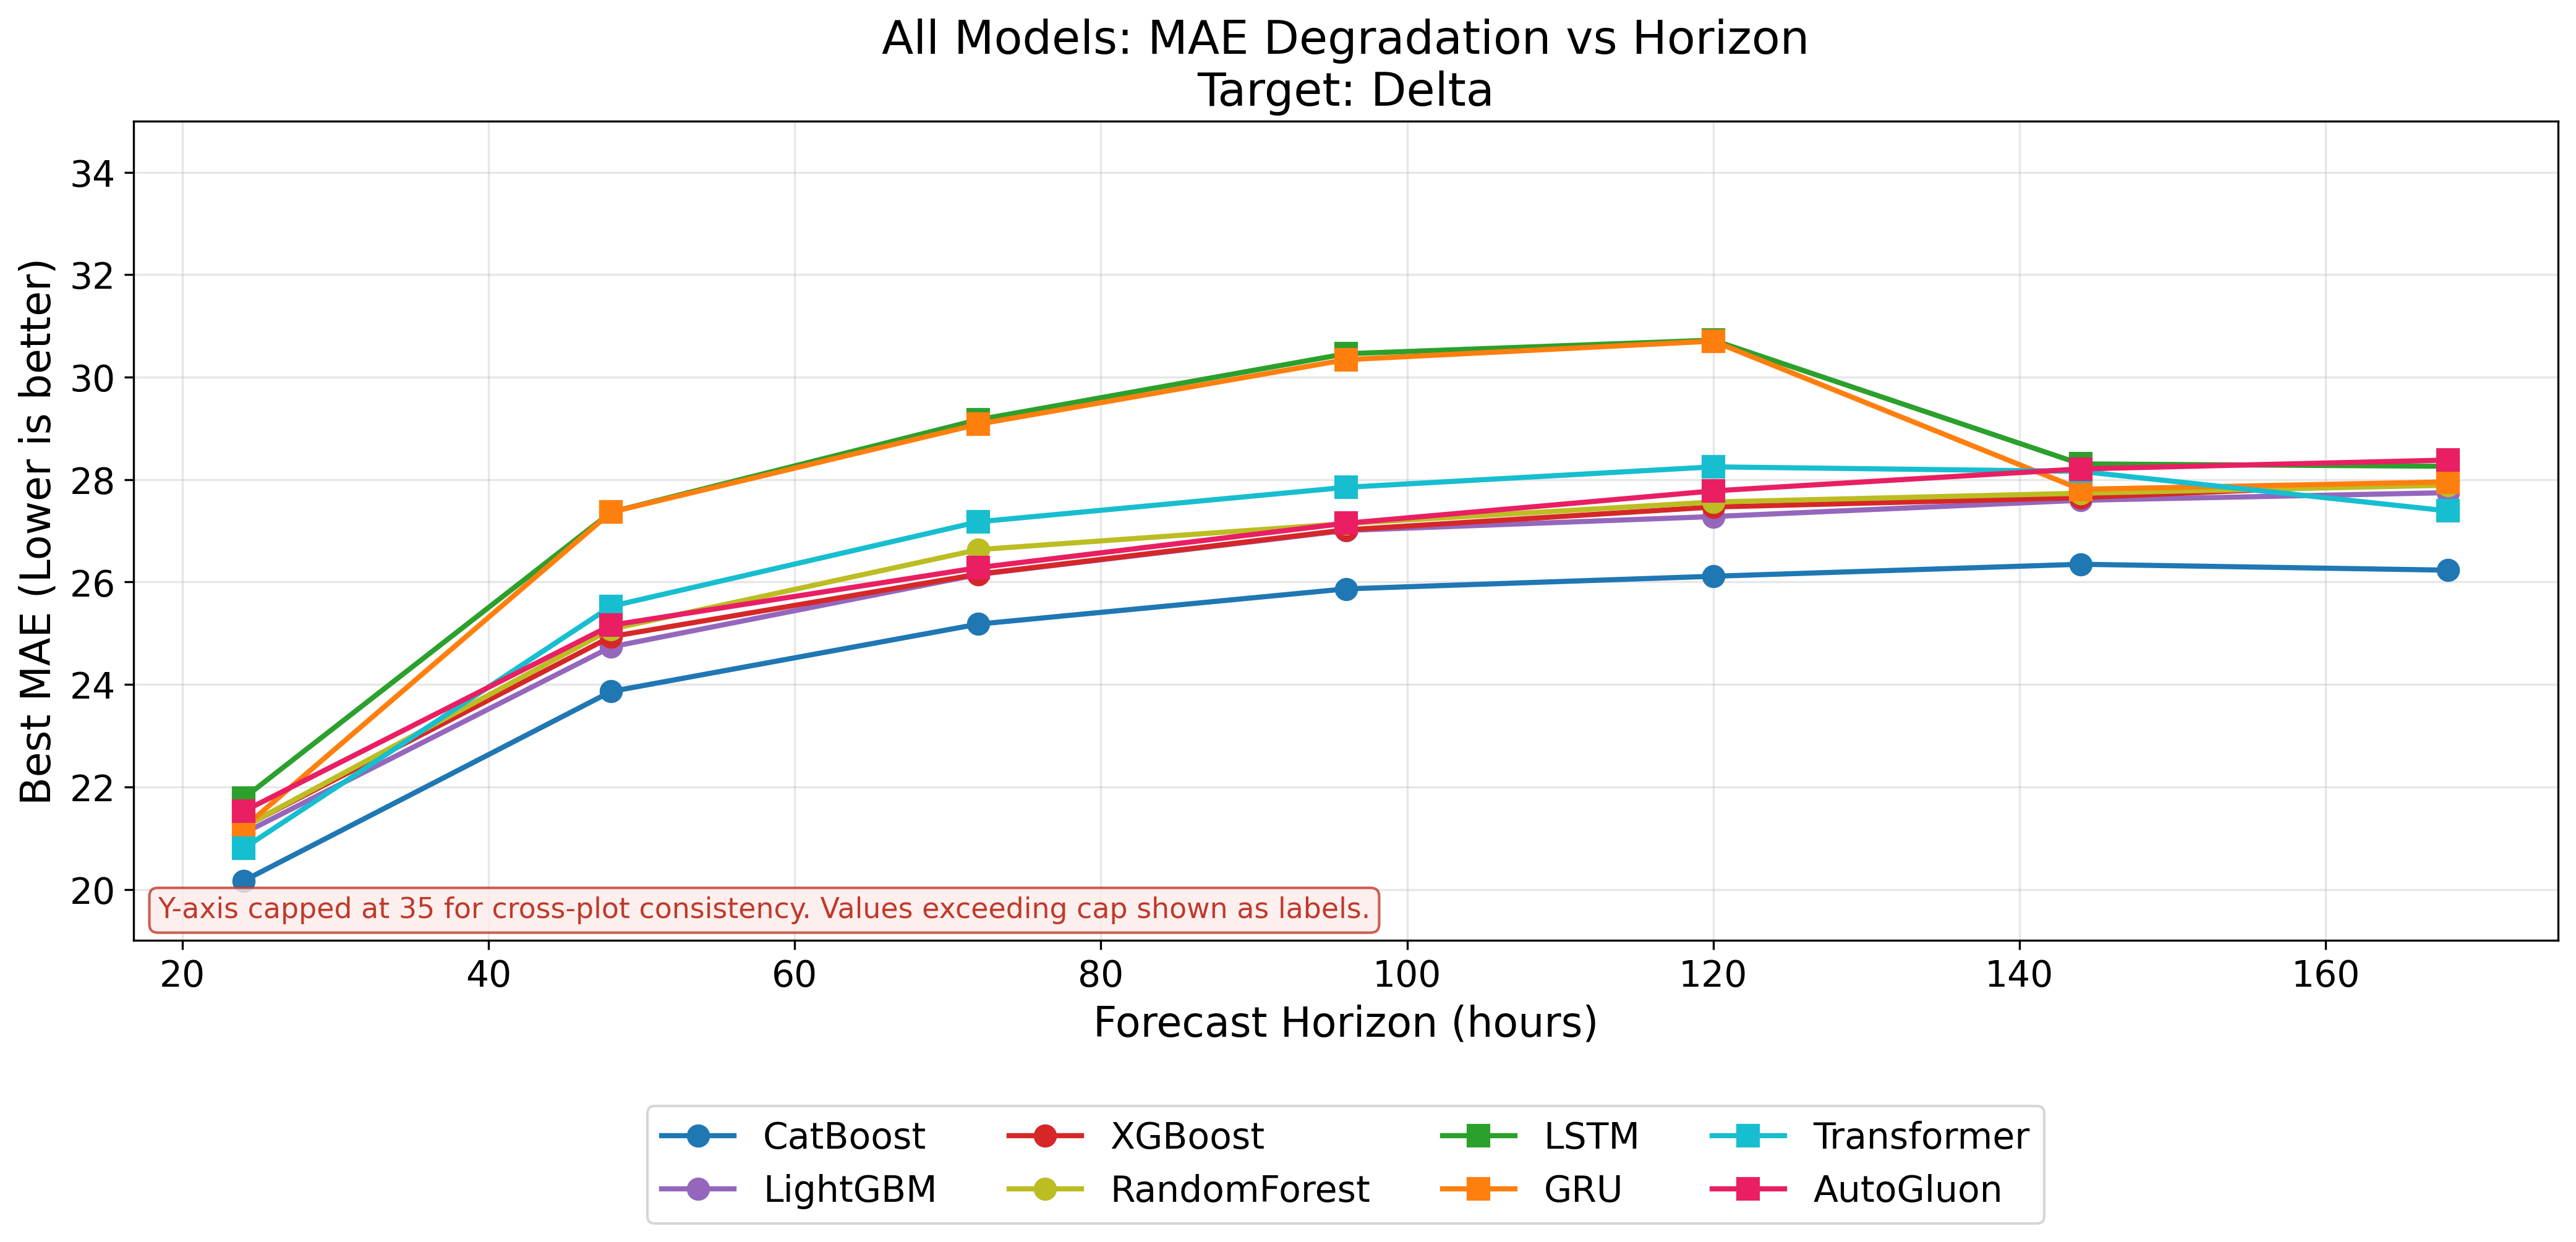
\includegraphics[width=\linewidth]{fig/Horizon_Degradation_All_Delta_MAE.png}
	\caption{Graph showing how each of the architectures degrade
		as the forecasting horizon is expanded. Lower is better.}
	\label{fig:horizonDegredation}
\end{figure}
One might expect that as the forecasting horizon is expanded
further into the future, that we would see a drastic drop
in predictive performance, however, \autoref{fig:horizonDegredation} shows us a
slightly different story. As can be seen in \autoref{fig:horizonDegredation}, 
while there is a drop in \gls{mae} across all models when expanding the
forecasting horizon, the differences in their degradation seems
mostly similar. Tree-based models and Gluon seem to be more
resilient to expanding horizons, but when approaching one week
into the future, the neural network-based models catch up in
performance. Additionally, the same drop in performance of
\gls{gru}, when predicting absolute price, can be seen in \cref{app:B}
\autoref{fig:modelComparisonPrice}.

\subsection{Feature importance}
This subsection relates to the feature importance analysis
that was performed through permutation importance. First we
look to which groups of features, in general across all models,
were the most impactful in contributing to low \gls{mae} scores.
Afterwards, we look to whether removing features that did
not significantly contribute to MAE would increase the overall
performance after pruning.

\subsubsection{Most impactful features}
\begin{figure}[t]
	\centering
	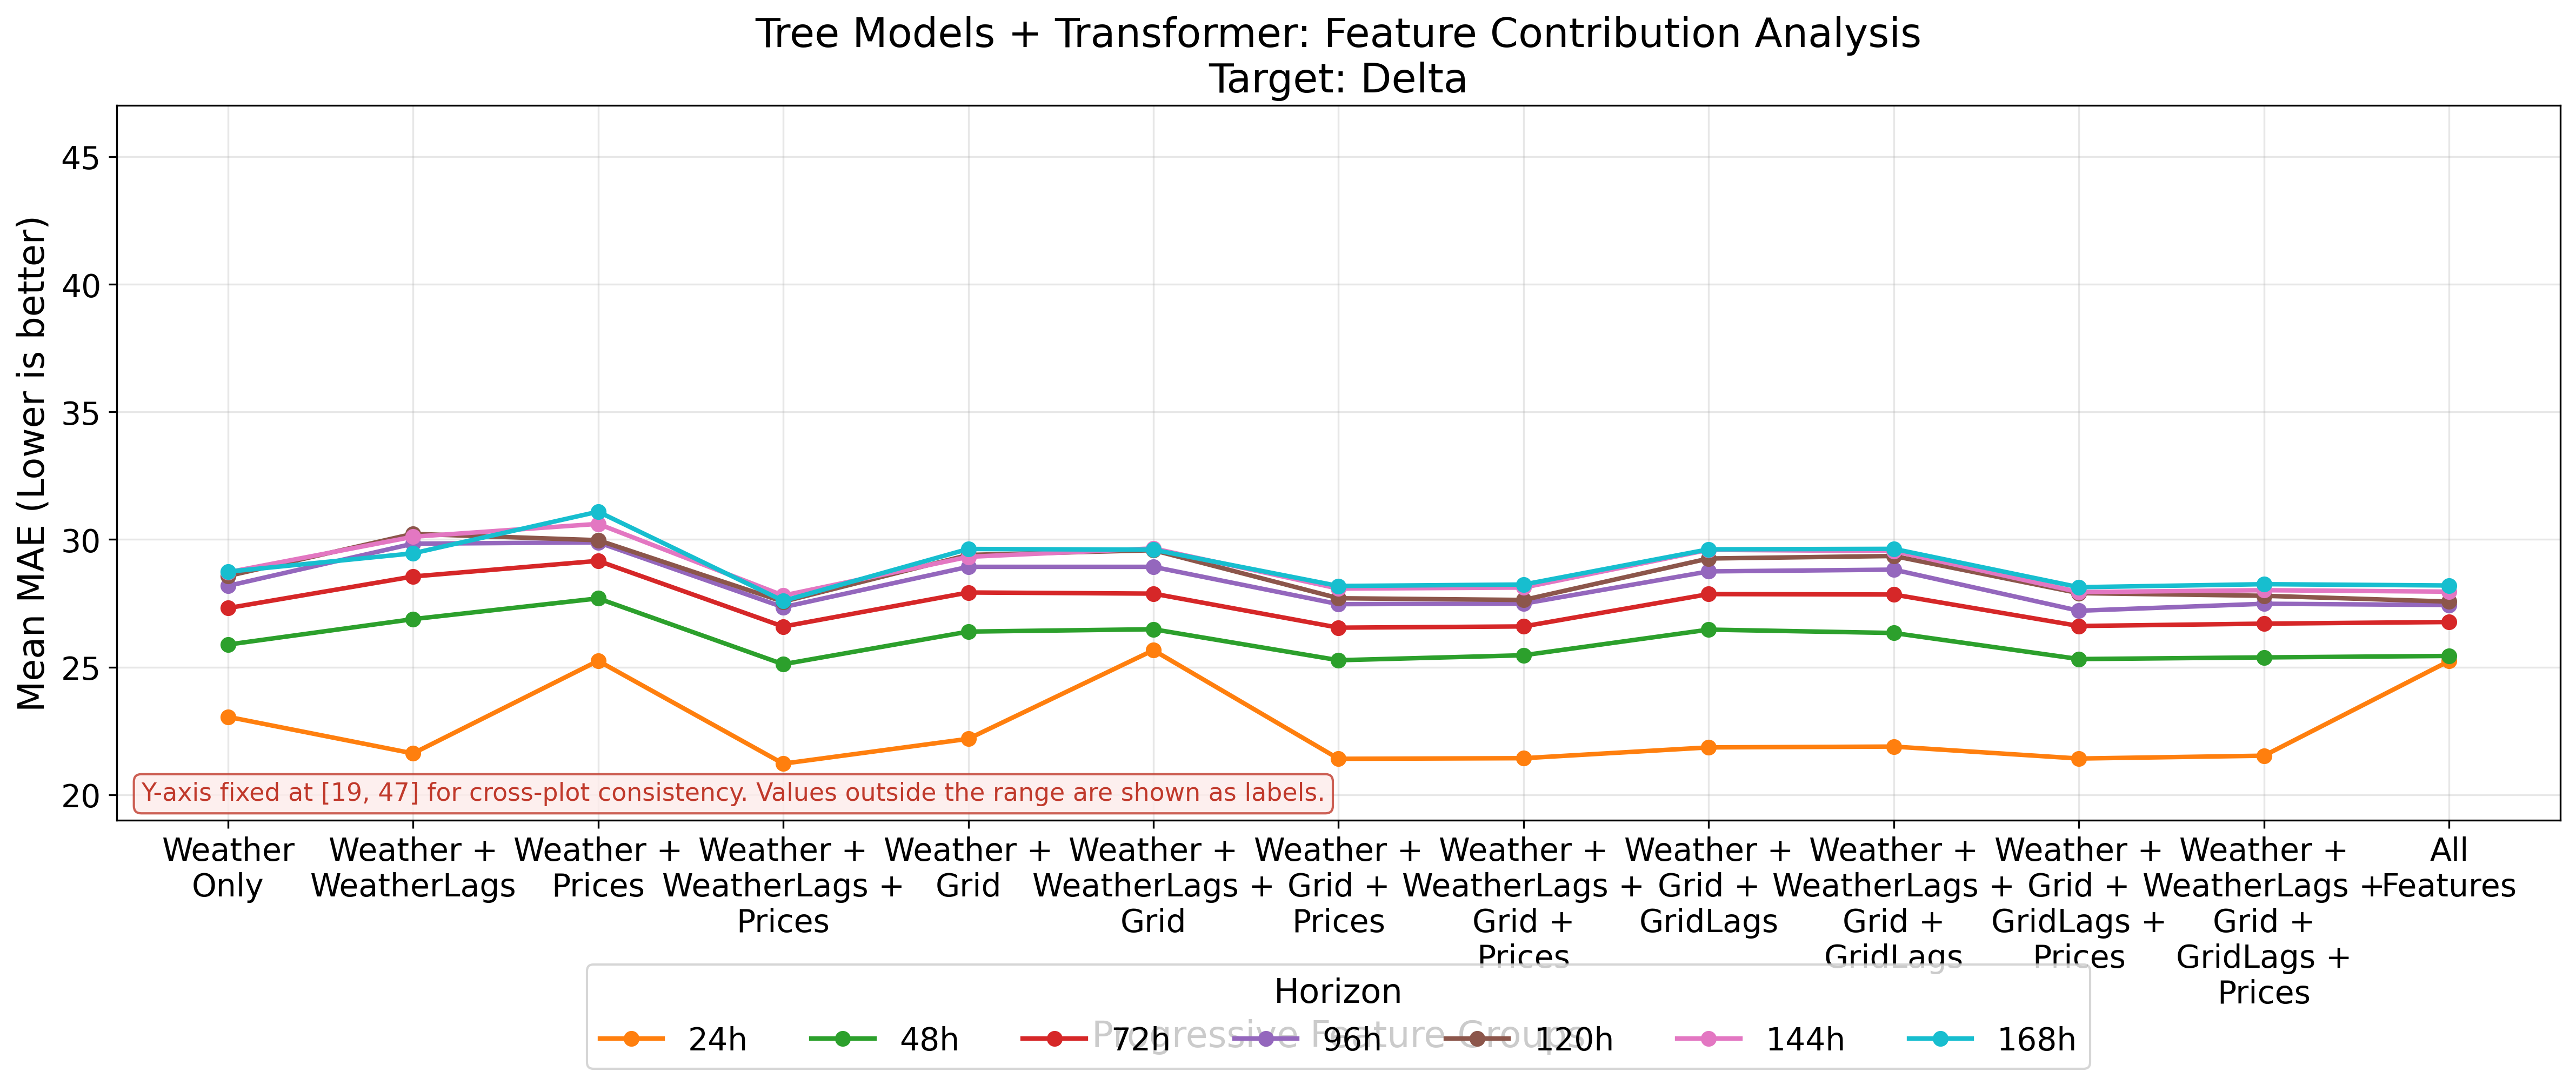
\includegraphics[width=\linewidth]{fig/Feature_Contribution_Combined_Delta_MAE.png}
	\caption{Graph showing the average MAE of all models across
		a given horizon and experiment-group combination with delta
		as the target. Lower is better.}
	\label{fig:featureContributionDelta}
\end{figure}
\begin{figure}[t]
	\centering
	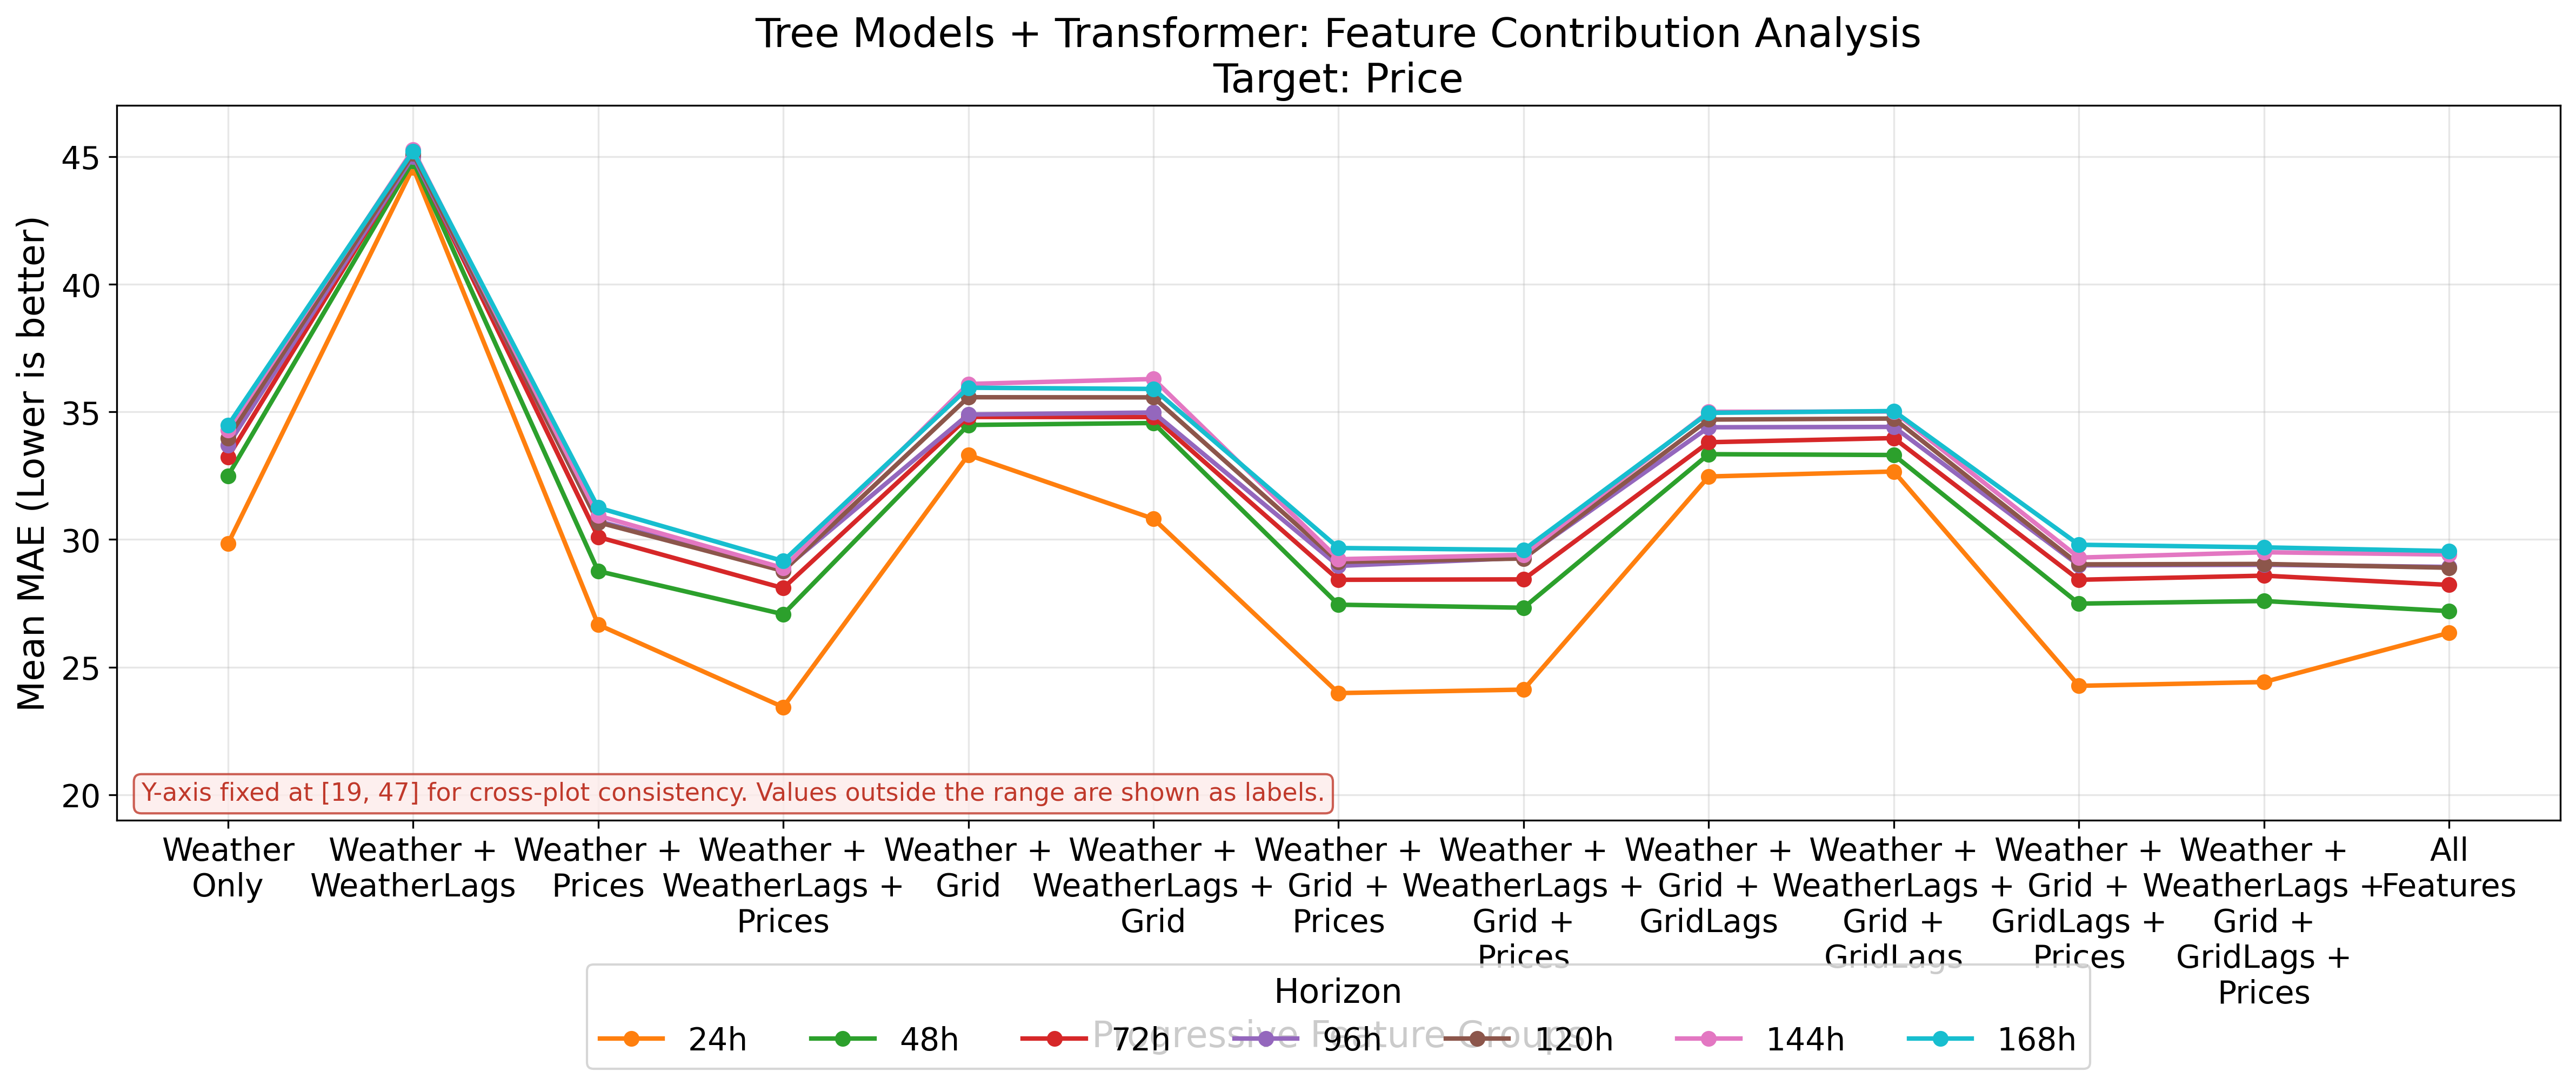
\includegraphics[width=\linewidth]{fig/Feature_Contribution_Combined_Price_MAE.png}
	\caption{Graph showing the average MAE of all models across
		a given horizon and experiment-group combination with price
		as the target. Lower is better.}
	\label{fig:featureContributionPrice}
\end{figure} 
As can be seen in both \autoref{fig:featureContributionDelta} and 
\autoref{fig:featureContributionPrice}, this is the first time that 
changing the target has a significant change in the behaviour of the models. 
This data suggests that utilizing delta as ones forecasting target makes
the models less sensitive to data compositions. The data also
shows that the further the forecasting horizon expands, the
closer the predictions cluster together, and that the sensitivity
to particular data-group constellations become less pronounced.

\subsubsection{Feature permutation}
\begin{figure}[t]
	\centering
	
\includegraphics[width=\linewidth]{fig/Pruning_Gain_Price_MAE.png}
	\caption{Visualization of pruning impact. Upwards bars indicate
		improvement in performance after pruning, while downward
		bars indicate a decrease in performance.}
	\label{fig:pruningGain}
\end{figure} 
With the knowledge that different data constellations impact the performance of 
models, feature permutation was performed, retaining columns whose removal
degraded \gls{mae} by more than 0.01 EUR/MWh, and the resulting
changes to each models can be seen in \autoref{fig:pruningGain}. The data shows
that feature permutation and pruning generally affected the
tree-based models negatively. This is not surprising, as it has
been previously mentioned that tree-based models are generally
well-equipped to innately filter out noise. Therefore, this drop in
performance may be the result of some features not improving
the MAE score by themselves, but in combination with other
such features they reveal hidden combined information that the
tree-based models utilise well. Fittingly, pruning almost always
improved the performance of the neural network-based models
and, in particular, seem to have largely mitigated the particular
noise sensitivity of \gls{gru}, as it saw particular improvements at
its struggling horizons. It is worth noting that pruning typically
produced results with a change of less than $\pm5\%$ in nearly
all configurations, suggesting that feature permutation offers
limited benefits at this scale. Readers are directed to 
\autoref{tab:pruning-delta} and \autoref{tab:pruning-price} in \cref{app:C}, 
should they be curious as to which specific experiments were pruned, and how 
many columns from each group were discarded.

\subsection{Supplementary experiments}\label{sec:resultsSupExp}
These last results relate to the supplementary experiments
discussed in \autoref{sec:expSupExp}. The following results of the
supplementary experiments shed light on the effects of various
methodological choices throughout the paper, as well as serve
to address additional methodological concerns. 

\subsubsection{Forecasting vs. baseline}
\begin{figure}[t]
	\centering
	
\includegraphics[width=\linewidth]{fig/Naive_Baseline_Comparison_Delta.png}
	\caption{Comparison of the MAE achieved by the baseline and
		the forecasted estimate. Lower is better.}
	\label{fig:naiveBaseline}
\end{figure} 
To determine whether it was
even worth it to try and predict electricity prices, the best
forecasting approach, CatBoost, was compared against a naive
baseline. This baseline was constructed by always predicting
yesterdays' price, no matter the horizon. As can be seen from
\autoref{fig:naiveBaseline}, forecasting exhibits particularly favourable 
performance at low 
horizons. As horizons escalate, the advantageous
margin diminishes, but remains in some measure for the totality
of the tested horizons. As this paper focuses on the ablation,
and not performance, these findings simply support that the
models tested in these experiments would still be of commercial
preference to simply re-using previous prices.

\subsubsection{DK1 vs. DK2}
\begin{figure}[t]
	\centering
	
\includegraphics[width=\linewidth]{fig/DK2_Generalization_Delta.png}
	\caption{MAE comparison between models trained on data from
		the DK1 and DK2 regions respectively. Lower is better.}
	\label{fig:DK1DK2}
\end{figure} 
As the Danish energy grid is divided
into two sections, DK1 and DK2, which differ significantly in
their geography, a small-scale experiment was conducted to
investigate whether the performance of models would change
depending on the region of their training data. \autoref{fig:DK1DK2} shows
that there are only small differences in the performance of both
models when trained on the DK2 region, compared to their
DK1 counterparts. However, the difference in performance is
slightly larger between the CatBoost models than between
the transformer models. This indicates that there may be
some factors that make DK2 a harder region to forecast
utilizing the CatBoost architecture, be it its smaller area, less
varied geography, or something else entirely. As it is not the
primary focus of this paper, such investigation is left for future
researchers to engage with.

\subsubsection{AutoGluon preset upgrade}
\begin{figure}[t]
	\centering
	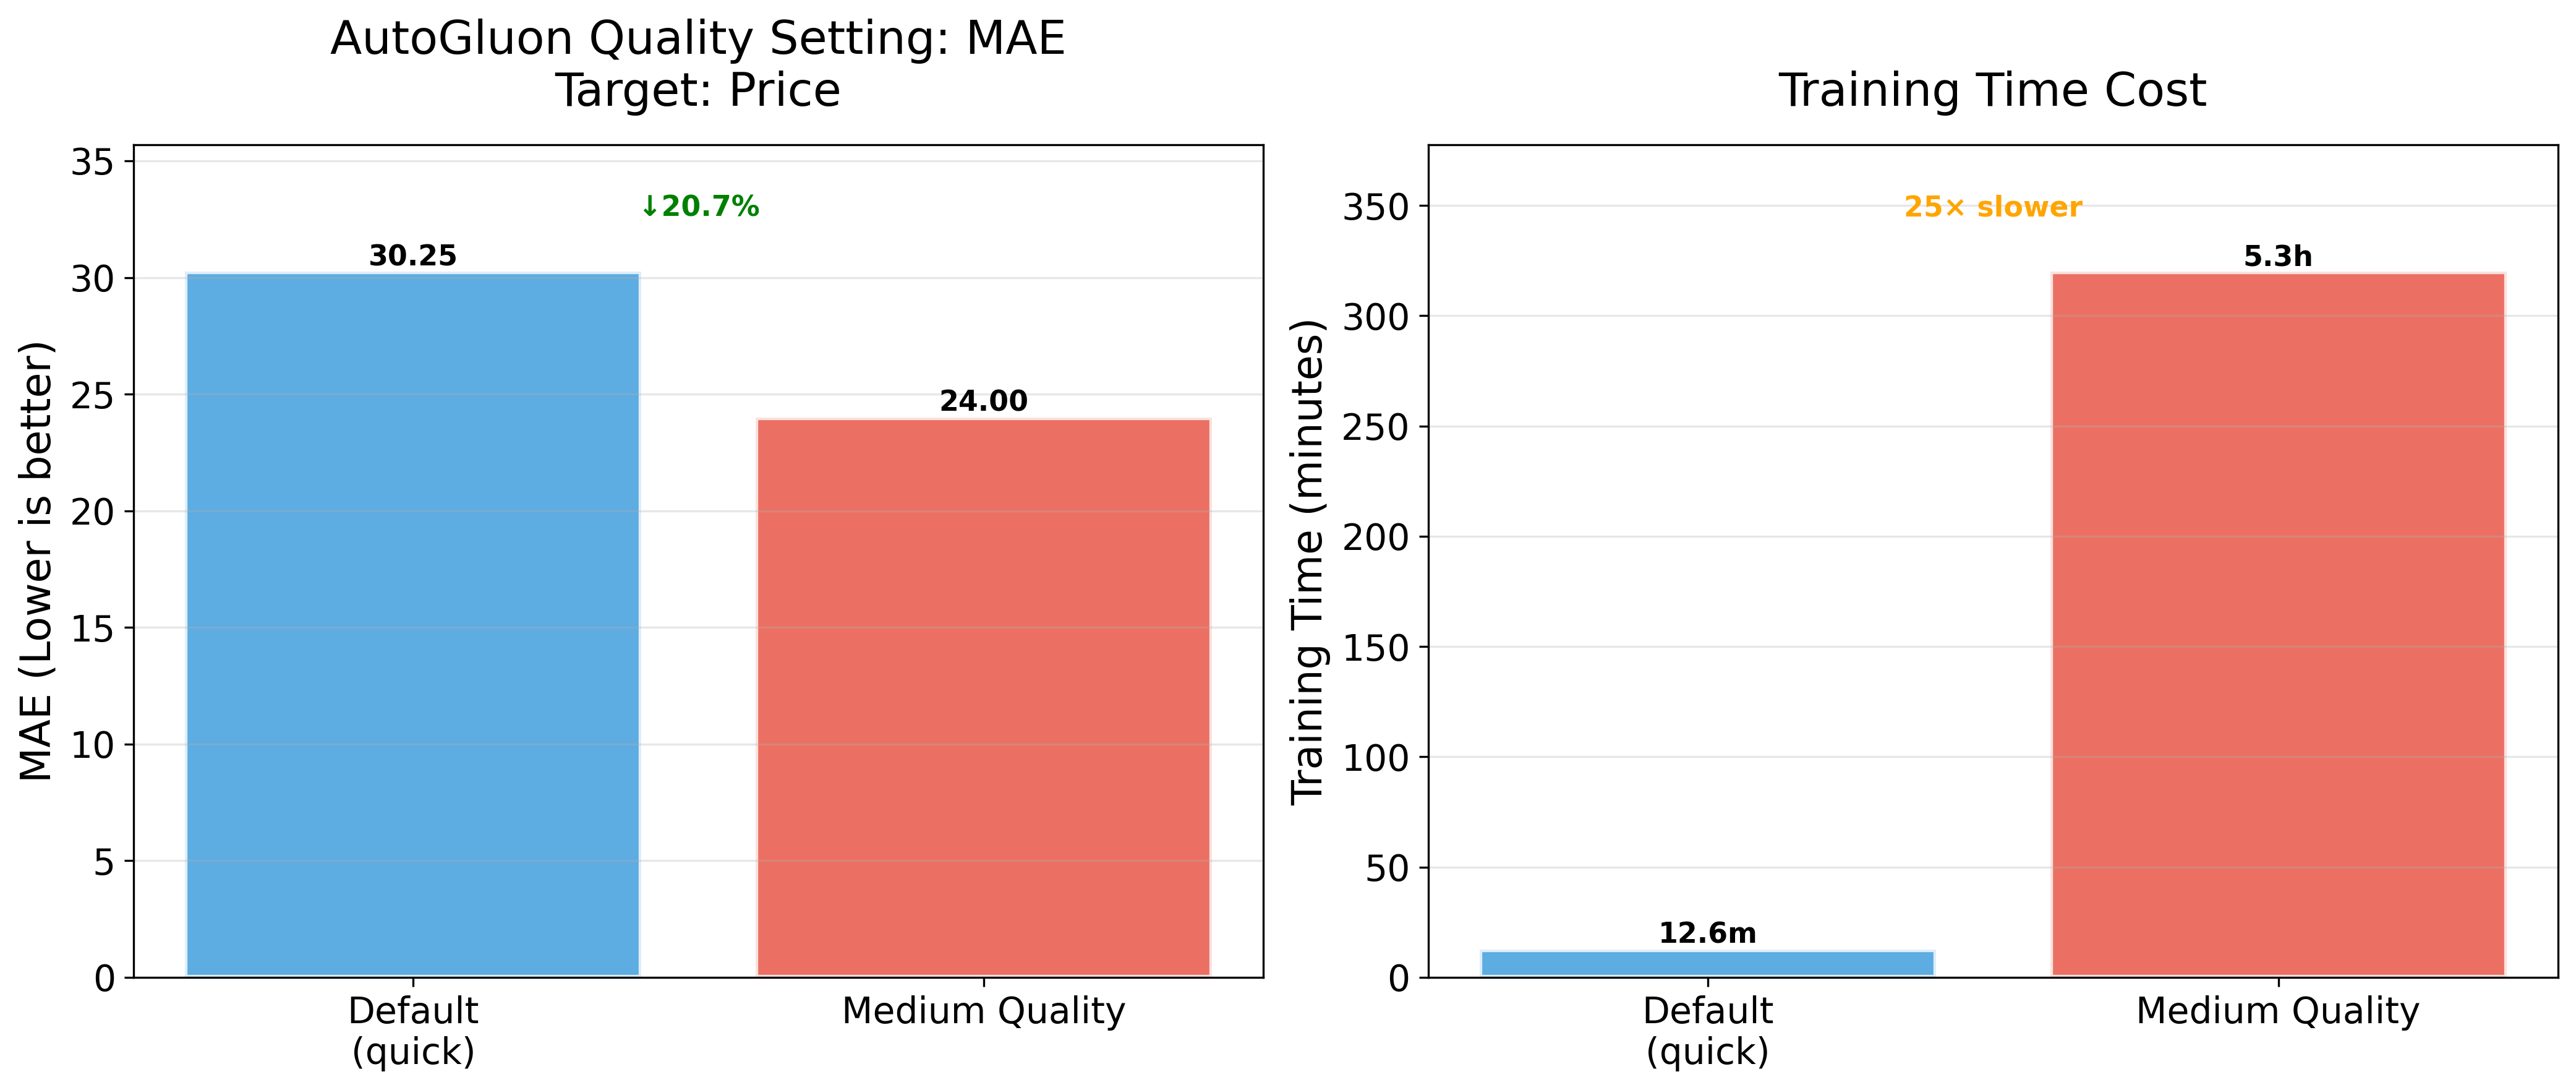
\includegraphics[width=\linewidth]{fig/AutoGluon_Quality_Tiers_Price.png}
	\caption{MAE and training time comparison between the fast
		and medium AutoGluon presets. Lower is better.}
	\label{fig:autoGluonPrice}
\end{figure} 
As previously mentioned, during the ordinary experiments Gluon was, due to 
time-constraints, run with its fastest preset. In this experiment, we
tried running it on the medium preset, as well as giving it 30
times more training time than it was previously allowed. As
depicted in \autoref{fig:autoGluonPrice}, there were performance improvements 
to be found by adjusting the preset quality of Gluon. However, it
is unclear whether such improvements would have been found
without the increase in training time as well, or how even higher-quality 
presets may affect performance. Such experimentation
is left for the reader. Additionally, it should be noted that the
improvement of 20\% was only applicable to the price target,
as the delta actually saw a slight decrease in performance, as
can be seen in \cref{app:B} \autoref{fig:autoGluonDelta}.

\subsubsection{Optuna hyperparameter tuning}
Hyperparameter tuning was performed for the tree-based models at the 24-hour
horizon, to gauge the impact it may have on the models'
performance. The results can be seen in \cref{app:B} \autoref{fig:optunaDelta} 
and \autoref{fig:optunaPrice}. We see that model performance normalises quite
heavily when comparing targets, with the 2 EUR/MWh gap
that was previously in the delta targets favour, being reduced
0.5 EUR/MWh at maximum. Further, we also see that the
competitiveness between the models is tightened, meaning that
the between-model gaps are closing as well. Lastly, we see that
any model that has undergone hyperparameter optimisation
outperforms all models that have run on their default settings.
This signifies that of all the tested models, one can easily make up for poor 
model selection by performing hyperparameter
optimisation.

\subsubsection{Loss function alteration}
\begin{figure}[t]
	\centering
	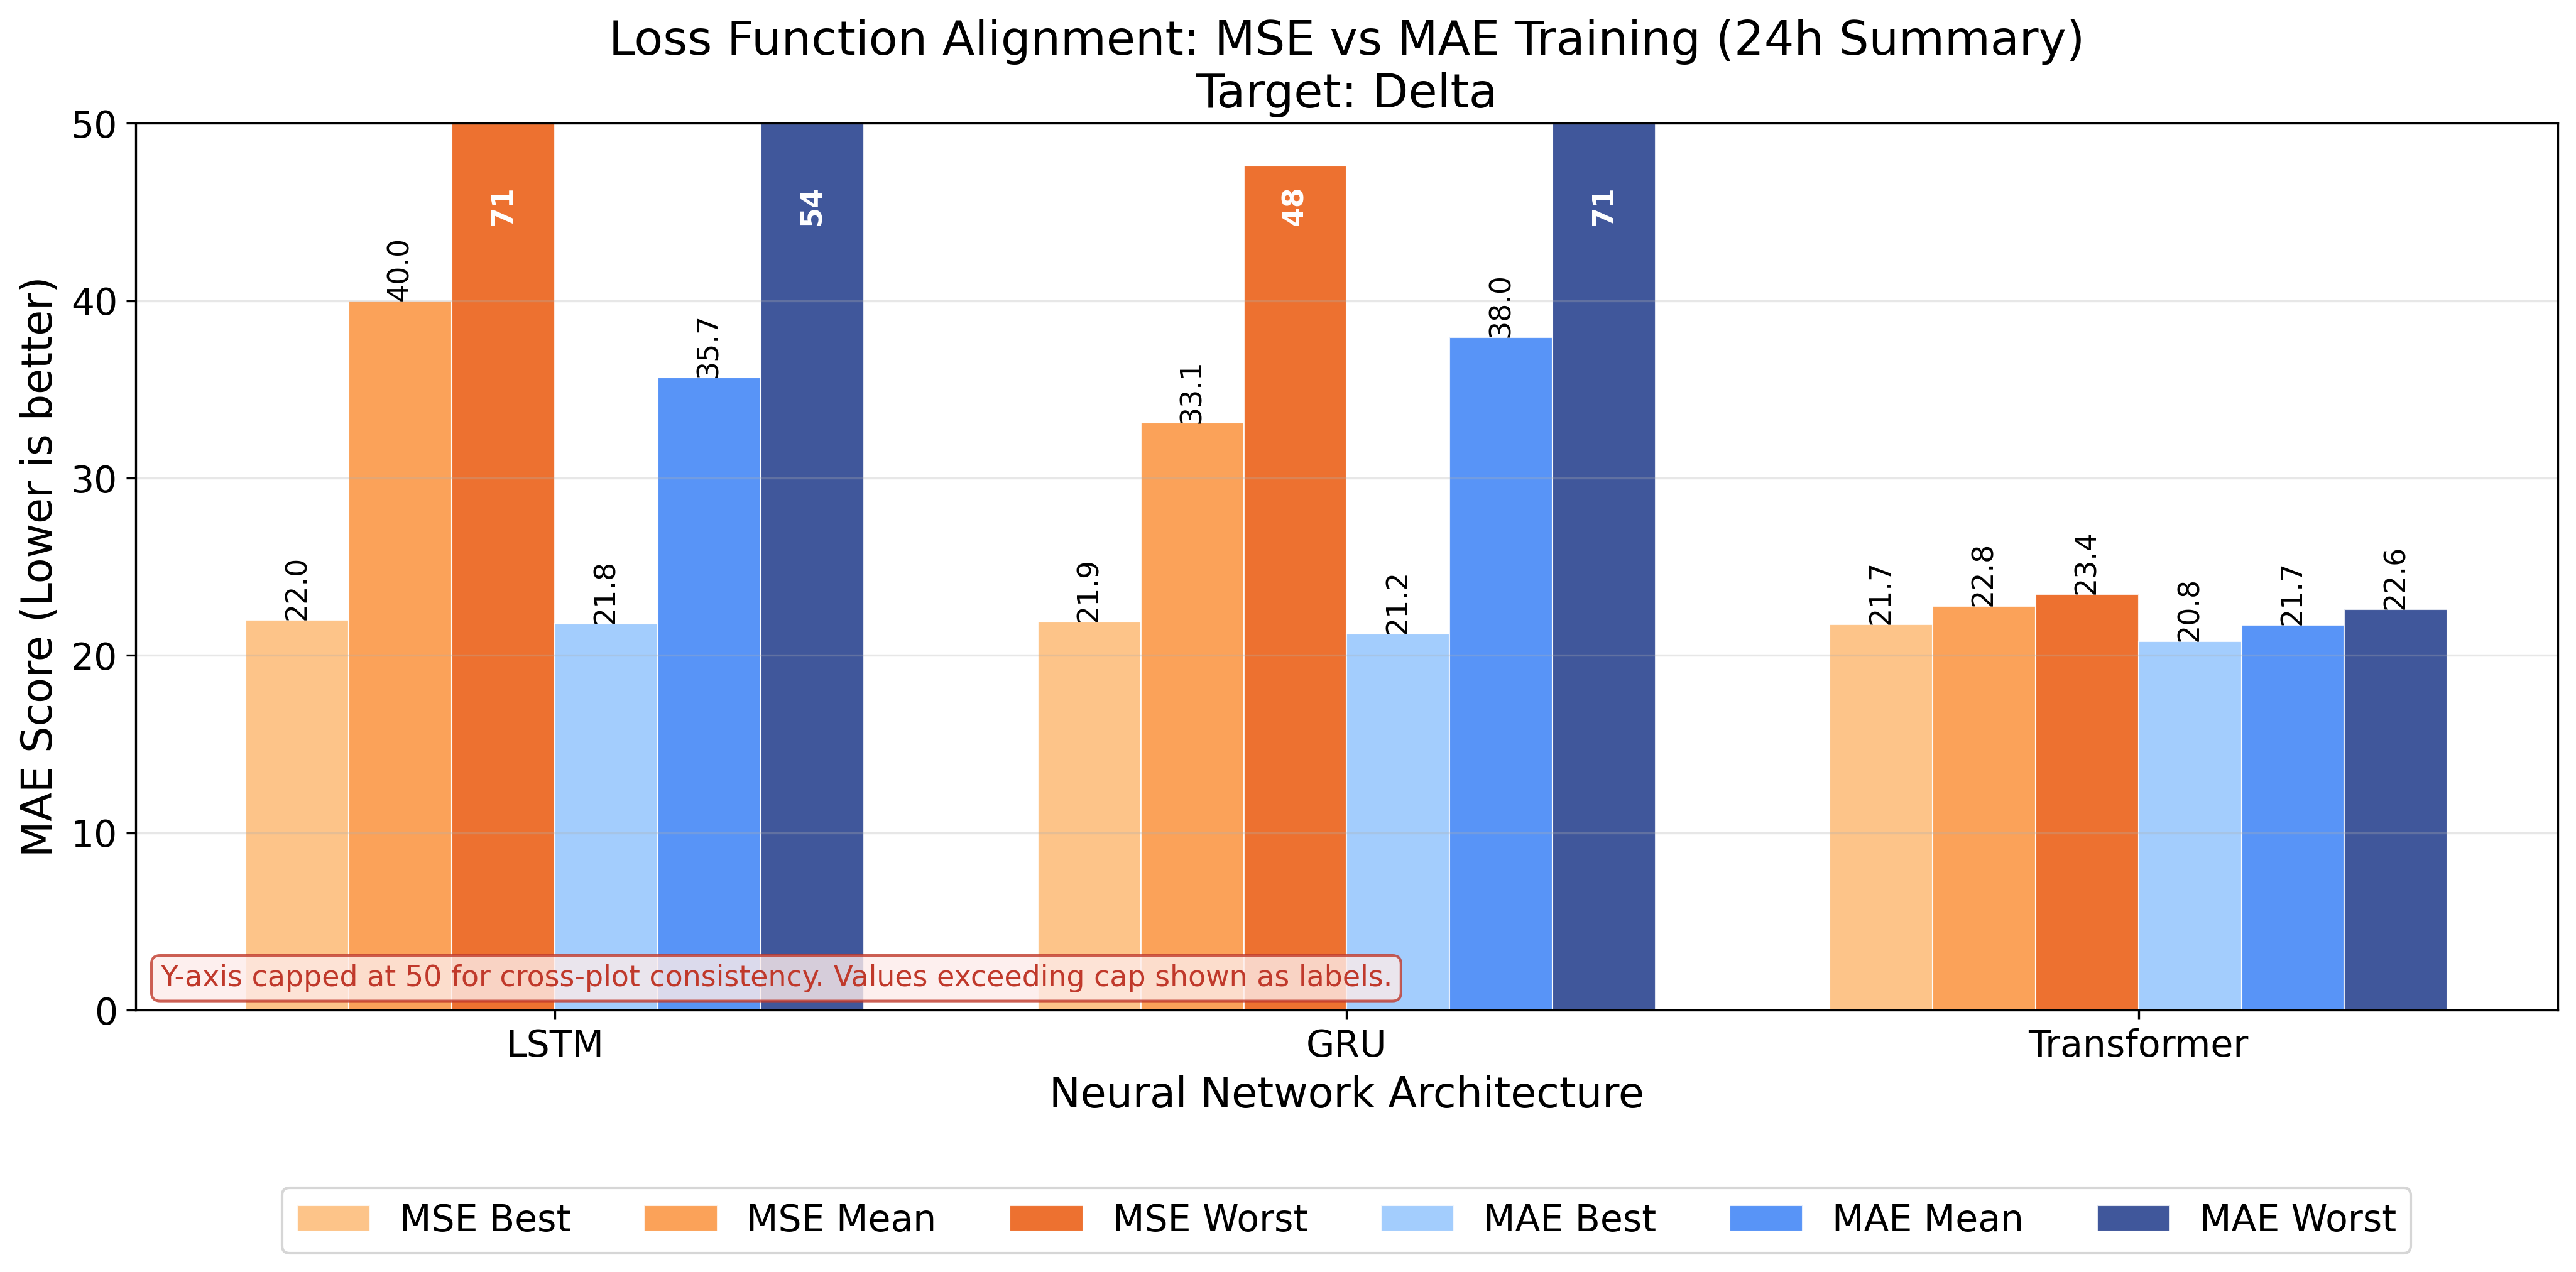
\includegraphics[width=\linewidth]{fig/Loss_Function_Summary_24h_Delta.png}
	\caption{\gls{mae} comparison of neural network-based models
		with \gls{mse} and \gls{mae}as loss functions. Lower is better.}
	\label{fig:lossFunctionAlignment}
\end{figure} 
Altering the loss function
from the standard \gls{mse} to \gls{mae} had both a significant, and
insignificant, impact on the neural network-based models.
As can be gleaned from \autoref{fig:lossFunctionAlignment}, there were 
significant improvements to be found in the mean and worst performing
neural network-based models, when switching from \gls{mse} to
\gls{mae} loss functions. However, it can also be seen that, while
there is slight improvement, the change in performance of
the best models was typically less than one EUR/MWh. In a
practical sense, this suggests that one may avoid many of the headaches that 
come with choosing the right data constellation
if one simply choses the correct loss function.

\subsubsection{Midas Energy data}
Lastly, the addition of- and substitution with Midas-prepared weather data to 
the models was investigated, to determine if its addition, or substitution with,
would positively impact the models at the 24h horizon. The
results of the addition can be seen in \cref{app:B} \autoref{fig:midasAddDelta} 
and \autoref{fig:midasAddPrice}. When adding Midas data to an already existing
dataset we see that when targeting delta, performance generally
decreased across all models. When targeting absolute price
instead, there were generally marginal improvements. So,
depending on the prediction target, it may be beneficial to
add professionally processed weather data into your dataset,
but the gain is not universal. To further investigate the impact
of Midas data, we instead constructed another experiment, with
all data ranging from 2021 to 2026, as that is the range of
availability of the Midas data. In this experiment, we substituted
all of the weather related columns, with the ones provided
by Midas. The results of this substitution can be seen in
\cref{app:B} \autoref{fig:midasSubDelta} and \autoref{fig:midasSubPrice}. These 
results show that there is no practical difference in the performance of runs 
with professionally processed weather data, and the data compiled
by this paper.
